\documentclass[11pt]{article}
\usepackage[margin=1in]{geometry}
\usepackage{graphicx}

%\renewcommand{\rmdefault}{phv} % Arial
%\renewcommand{\sfdefault}{phv} % Arial

% Dana found this online, but currently using geometry package

%%%%%%%%%% EXACT 1in MARGINS %%%%%%%                                   %%
%\setlength{\textwidth}{6.5in}     %%                                   %%
%\setlength{\oddsidemargin}{0in}   %% (It is recommended that you       %%
%\setlength{\evensidemargin}{0in}  %%  not change these parameters,     %%
%\setlength{\textheight}{8.5in}    %%  at the risk of having your       %%
%\setlength{\topmargin}{0in}       %%  proposal dismissed on the basis  %%
%\setlength{\headheight}{0in}      %%  of incorrect formatting!!!)      %%
%\setlength{\headsep}{0in}         %%                                   %%
%\setlength{\footskip}{.5in}       %%                                   %%
%%%%%%%%%%%%%%%%%%%%%%%%%%%%%%%%%%%%

% old

%\oddsidemargin=0in
%\textwidth=6.5in
%\textheight=9in
%\topmargin=-.625in

\linespread{1.4}

\begin{document}
\begin{center}
{\Large \textbf{Collaborative Research: Resource of Open\\
Problems for Education (ROPE)}}
\end{center}

\begin{section}{Introduction}

At the heart of teaching and learning mathematics---and many other
disciplines---is a learner's engagement with questions, or problems, which
challenge her or him to understand and apply the material s/he is
learning.  We propose to develop a resource that will provide an on-line
electronic library of innovative, well-tested and documented problems that
instructors and students may use in a wide range of courses and for a wide
range of assignment types.  This ``Resource of Open Problems for
Education'' (ROPE) will allow searching and browsing to find appropriate
problems; will include descriptive information about problem usage and the
numbers of users endorsing the problems; and will allow users to share
problem collections and lists drawn from the library.  Because it will be
an open resource, institutions and individuals with limited means will
still have full access to it, and the community of ROPE users will be able
to provide added value to the library.  The goals of ROPE are:
\begin{itemize}
  \item
    To be a \textit{free, open-source resource} that will give instructors
    and students access to an extensive collection of good mathematics
    problems.  The cost of textbooks and supporting materials for courses
    is increasingly untenable.  We believe that as academics
    we should work to have accessible resources that do not
    discriminate on the basis of wealth and which do not demand
    advertising or private data for their use.
  \item
    To have within this resource a mechanism for users to create
    \textit{collections of problems, and collections of collections,} 
    that they may use themselves or share with other users.
    This will allow instructors to create problem sets, quizzes, and
    collections of these for a course, will allow authors to define groups
    of problems that complement their text, and will allow students to create practice
    worksheets or other study aides.  This flexibility in use and
    sharing of collections will allow more and better use cases for the
    resource. 
  \item
    To provide ways to establish a \textit{community of users} of these
    problems, who may contribute problems and related content, may provide
    feedback on problems, and may share with other users the collections
    they have created.
\end{itemize}

\end{section}

\begin{section}{Description}

Internet users go to Amazon to search for material products to buy, and to
Google to find pages on the Internet.  While we do not pretend to be
creating a resource with the ubiquity or power of either of those, we do 
hope to develop ROPE into the place where mathematics teachers and
learners go to find problems and inspiration for problems for the courses
they are teaching and learning.  We imagine going to the ROPE search page,
such as is suggested in Figure~\ref{rope1}, and searching for a topic or
problem, with the result suggested in Figure~\ref{rope2}.  These mock-ups
illustrate a number of the core features that ROPE will have:

\begin{figure}
\begin{center}
\framebox{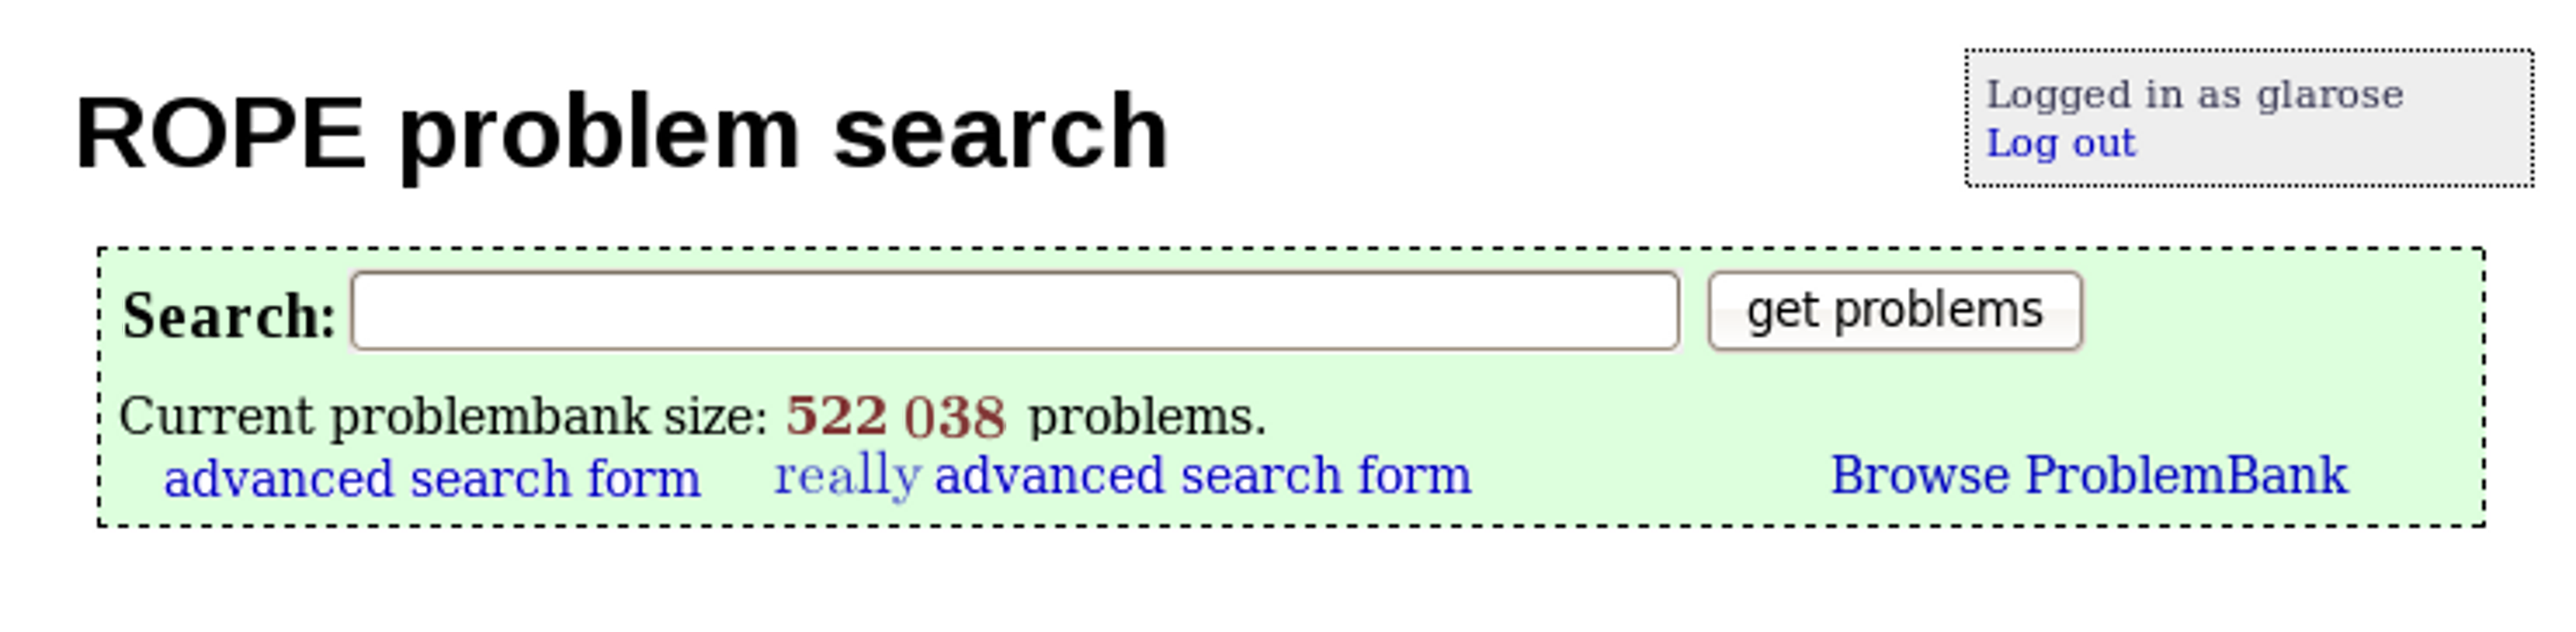
\includegraphics[width=5in]{rope_search}}\\
\caption{Mock-up of ROPE search page}
\label{rope1}
\end{center}
\end{figure}

\begin{figure}
\begin{center}
\framebox{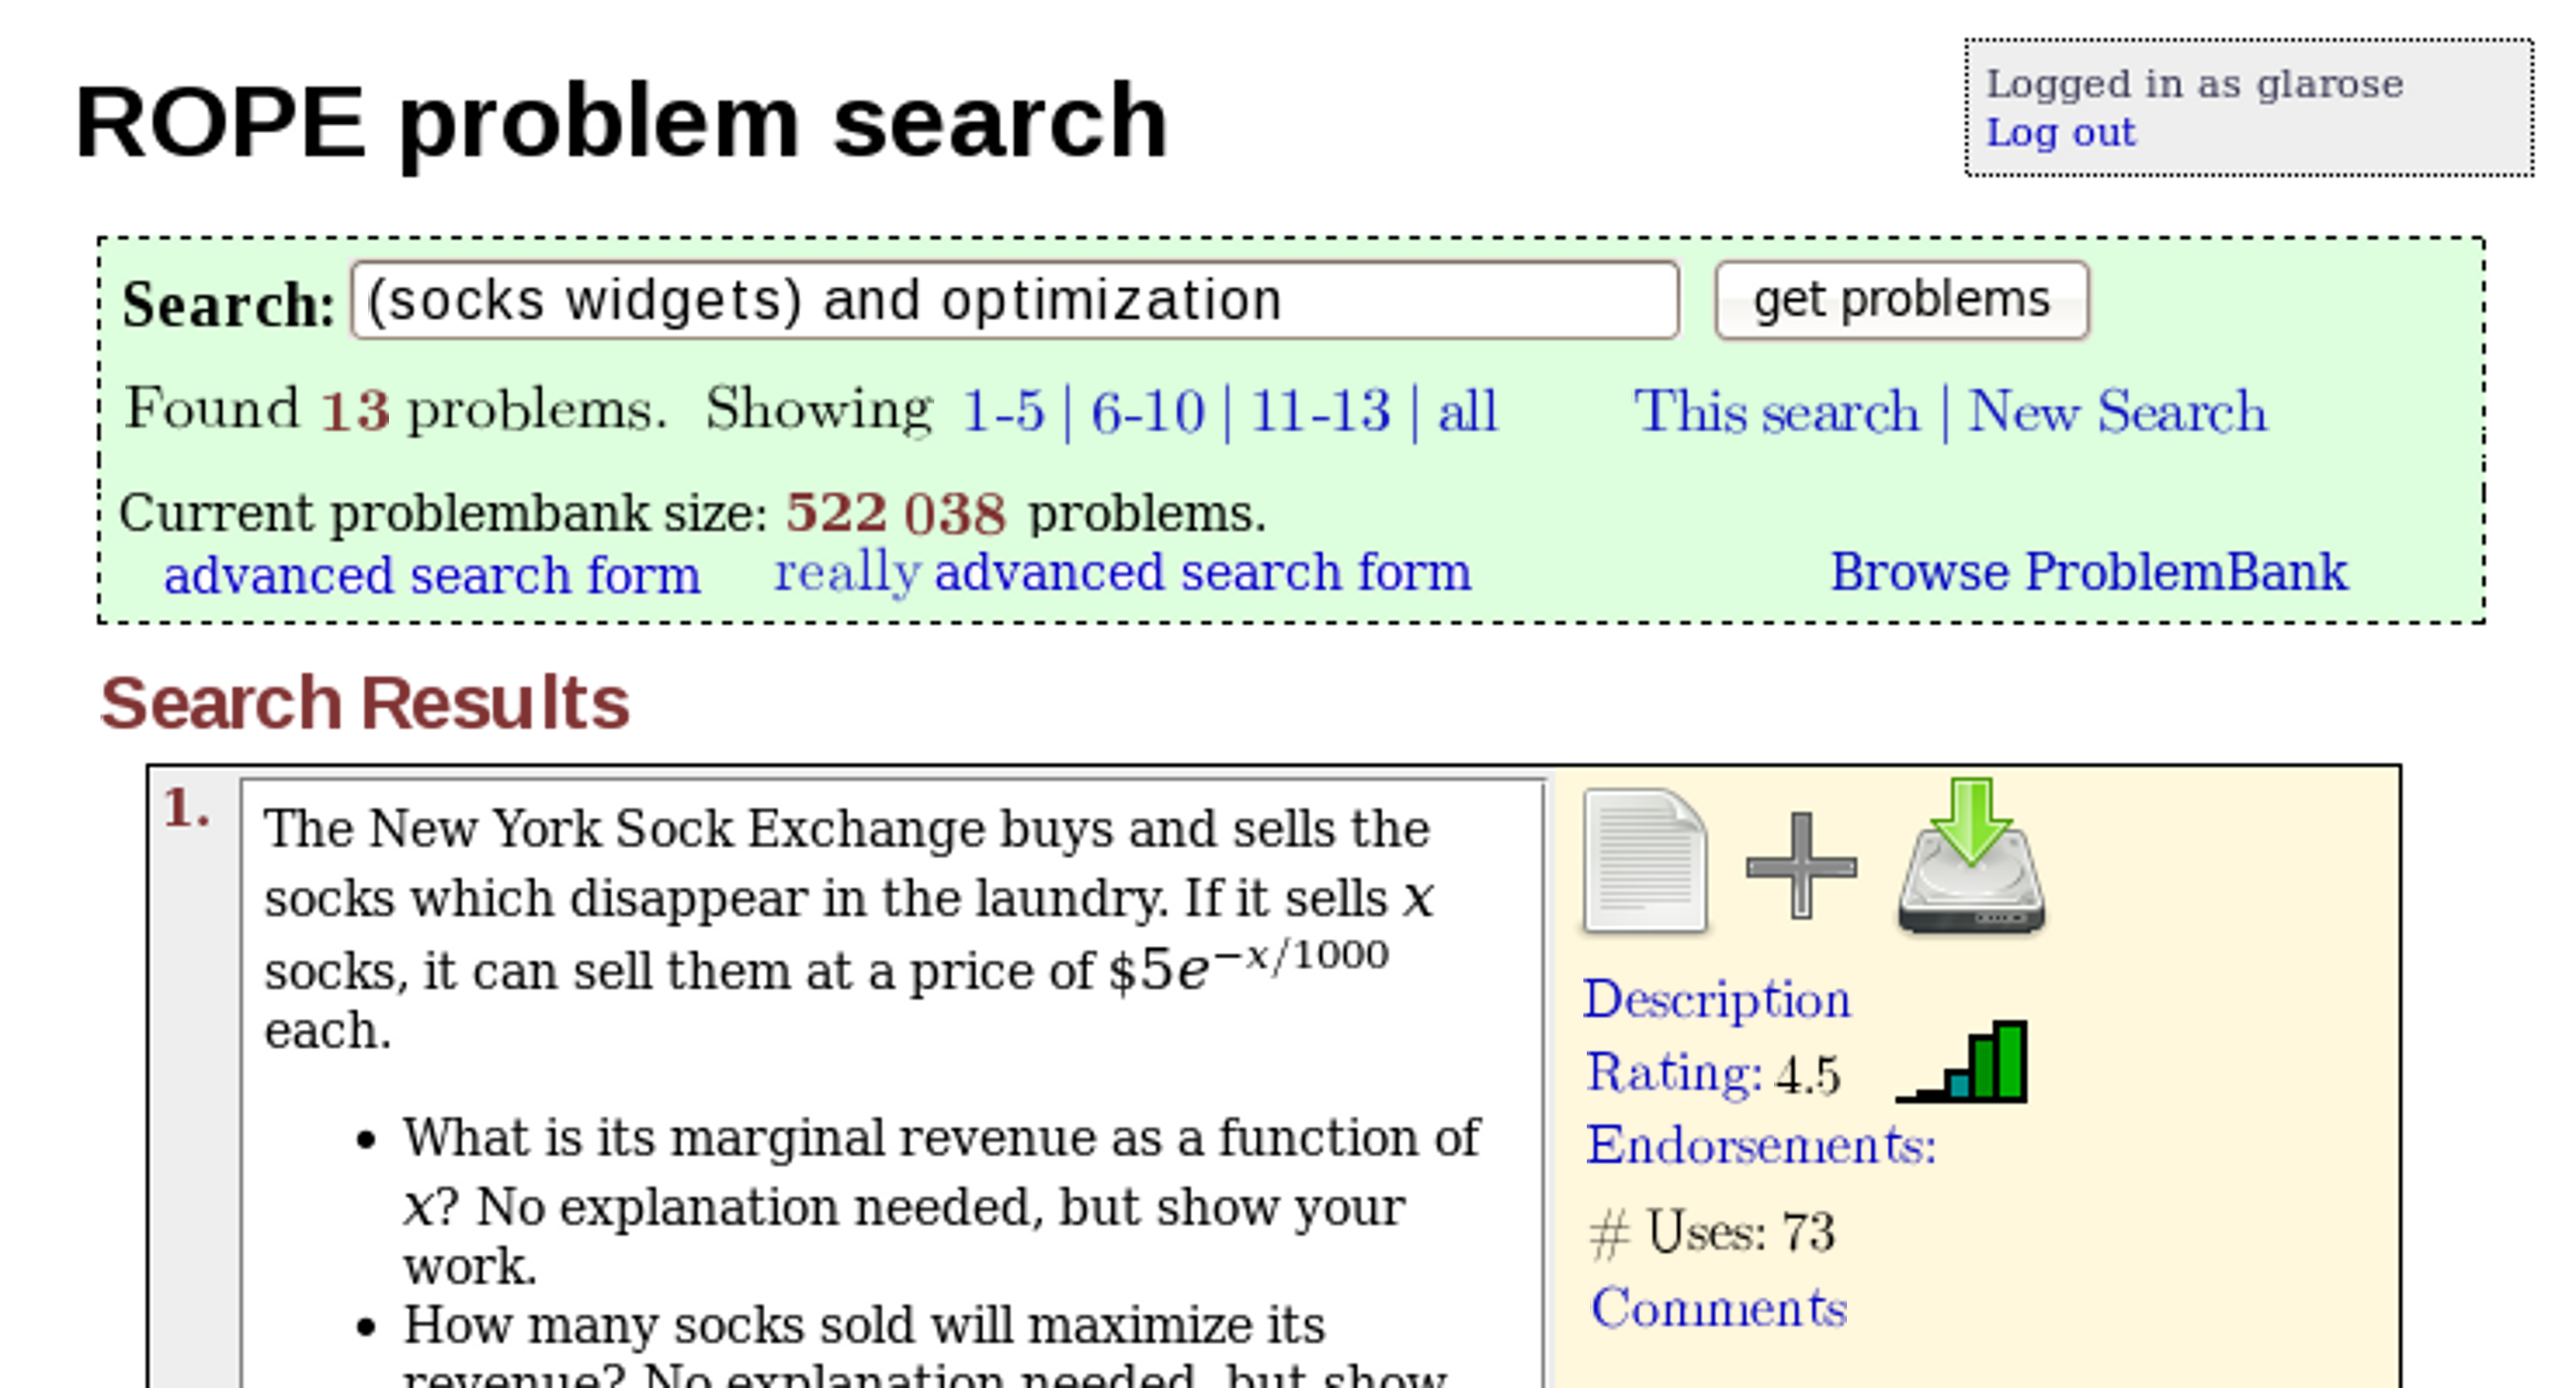
\includegraphics[width=5in]{rope_search_results}}\\
\caption{Mock-up of ROPE results page}
\label{rope2}
\end{center}
\end{figure}

\begin{list}{$\bullet$}{\setlength{\parsep}{0pt}\setlength{\itemsep}{0pt}}
  \item
    Users will be able to search on arbitrary keywords, or with GMail or
    Google-like tags (e.g., ``course:calculus'').
  \item
    There will be alternate search forms that will allow users to
    explicitly select specific courses, chapter or section headings, etc.
  \item
    Search results will be easily managed, with a view of the problems and
    easy ways to view the source (e.g., \LaTeX) for the problems, add them
    to Problem Collections owned by the user, or download the
    source as a small file.
  \item
    All problems will have useful metadata that describe them, including
    the background mathematics required for the problem (e.g., calculus
    and optimization), level of difficulty (e.g., easy, medium, hard),
    type of problem (e.g., symbolic, numerical, graphical), etc.
  \item
    Users will be able to rate problems, endorse them, and leave comments,
    and these data will be available to allow other users to evaluate the
    problems and how they might be used.
  \item
    Users will have the ability to build their own problem collections and
    share them with other users (as they like), and thereby download a
    full source file (e.g., in \LaTeX) for a problem set, other
    assignment, or even full list of all problem sets for a course.
\end{list}

In the following we discuss the three key functionalities we envision for
ROPE: the searchable problem library, from which users may view and
download problems; the ability to create collections and 
collections of collections; and its community of users and how that will
integrate with the other two features.  In a final section we discuss some
of the extensions and technical details that we expect to make ROPE as
flexible, useful and usable as possible.

\begin{subsection}{Searchable Problem Library}

We envision that instructors will come to ROPE to find problems for
homework or quizzes; or students will come to look for problems for review
or practice; or authors will come to create collections of problems to
augment those they have in their text; etc.  To serve these varied
communities and needs, we need to have a large collection of problems that
may be searched on multiple criteria.  Therefore, all problems in the
resource will be tagged to make it easy to find problems associated with a
course or course-topic, type of problem (e.g., one that requires graphical
understanding), and other characteristics.

Once problems are found that a user wants to use, s/he will be able to
view or download the substance (e.g., \LaTeX\ code) for the problem, or
add it to a collection of problems in ROPE that s/he has created.  When
viewing the problems, s/he will have access to the complete description of
the problem as it has been entered into the ROPE database.  This
description will include information such as that indicated in
Table~\ref{metadata}.  It will be possible to search on these fields, or
in the text of the problems themselves.

We expect that most of the problems in ROPE will be coded as \LaTeX\ code
snippets, because that is the most commonly used mark-up for mathematics
documents.  However, because this is not uniform, ROPE will
support other formats, e.g., small \emph{Word} or \emph{OpenOffice}
document files.  Where possible, our goal will be for it to be possible to
convert between formats when viewing or downloading problems; this is
addressed in greater detail below, in section 2.4.

\begin{center}
\begin{table}
\begin{tabular}{|l|l|}
  \hline
  \textbf{Characteristic} & \textbf{Description} \\
  \hline
  Author & Some identifier of the author, e.g., username \\
  Date   & An indicator of the date the problem was authored \\
  Difficulty & e.g., easy, medium or hard \\
  Type & e.g., symbolic, numerical, graphical, or multiple \\
  Course & An indicator of the course in which the problem might be used \\
  MajorTopic & ``Chapter'' level topic categorization \\
  MinorTopic & ``Section'' level topic categorization \\
  RelatedProblems & Other problems in ROPE with which this is associated \\
  RequiredTech & Technology required to solve the problem \\
  Keywords & Specific keywords describing the problem \\
  \hline
\end{tabular}
\caption{Metadata describing ROPE problems}
\label{metadata}
\end{table}
\end{center}

\end{subsection}

\begin{subsection}{Collections of Problems and Collections}

Any user of a problem resource is unlikely to use a single problem and
then stop.  We anticipate that most users will be looking for groups of
problems to use on quizzes, homeworks, study sheets, or to complement
different sections of their textbook.  ROPE will therefore support the
definition of such collections by its users.  The simplest such collection
would be a list of problems, such as might appear in a problem set, study
guide or quiz.

In addition, a collection in ROPE may contain other collections and
textual metadata.  Thus, a user may construct a collection of problem sets
for a course that s/he is teaching, or may construct a collection of
problem sets with embedded information that provides context (e.g., the
textbook being used, or the expectations for the ordering of material,
etc.) for her/him when s/he returns to use the sets again, or for others
with whom s/he shares the collection.

The ability to define such flexible and extensible sets also allows 
textbook authors (for texts published by a standard publisher, or for
authors of open-content texts) to establish collections of problems to
complement the text.  These collections could then be shared with any user 
who is using the text.  We hope that this will be an invaluable resource
for authors of open-content textbooks, and other authors creating problem
sets to complement their texts, and instructors interested in sharing
resources.  One immediate application of these collections in ROPE will be the
ability to share complete problem-centered course notes.  An increasing
number of instructors are using Inquiry Based Learning (IBL) in their
classrooms, for which course notes most commonly consist of problem sets
with some context and other information.  This type of collection of
materials will be very easy to create and distribute through ROPE.

\end{subsection}

\begin{subsection}{Community of Users}

Users of ROPE will be able to use the problems in the resource, build
their own collections of problems, and add to it.  Integral to our vision
for ROPE is that users will be active in contributing problems, rating
problems that exist, and providing valuable feedback to other users about
problems and how they may have been effectively used.

As suggested in the mock-up results page (Figure~\ref{rope2}), users will
be able to rate problems, and endorse them.  They will also be
able to use comments about the problems that may be useful to other
users.  As users create problem collections that they share
with other users, they will be making connections within the community
that will provide further added value to the resource.  

We will develop an easy-to-use interface through which 
users will be able to contribute
problems to ROPE.  The grant PIs will work with an advisory group to
determine the best model for moderation and vetting of contributed
problems, and to cultivate a user base that will end up forming the
community that we imagine.

\end{subsection}

\begin{subsection}{Extensions and Technical Details}

There are a number of things that a problem database such as ROPE should
include.  These include: flexibility to support different problem formats
and types; format conversion utilities that allow problems to be converted
between formats; and a well-documented API that will allow other
applications to communicate with ROPE in manners other than through the
browser interface.

As we indicate above, we expect that most mathematics problems will be
coded in \LaTeX\ snippets, but that there will be users for whom this will
not be appropriate.  ROPE will therefore support other formats such as
small \emph{Word} or \emph{OpenOffice} files, plain text, and we expect
other formats as well.  In particular, problems in PGML (a mark-up
language used for some WeBWorK problems), PG (the standard WeBWorK mark-up
language), and similar formats would be easy to include.  ROPE will also
support web-native problems that may be displayed on-line
directly, which will allow connections with other on-line applications.
This will allow an easy interface to \emph{Sage}, an open-source
mathematics program that may be used through an on-line interface.  We
will work with our advisory group to determine other formats that ROPE
should support, and determine how this may fit into the technical
framework that underlies the application.

Of course, if users can submit problems in a variety of formats, the resource 
must be able to convert between these formats.
%Given a variety of formats, of course, for the resource to be as useful as
%we envision it must be possible to convert between formats.  
A user of
\emph{Word} may not find \LaTeX\ snippets tremendously useful, for
example.  We will therefore support conversion between formats, insofar as
that is possible, and generation of generic intermediate formats (e.g.,
plain text) where it becomes prohibitively difficult.  This will allow
users with all different backgrounds to find and use problems regardless
of the format in which they were originally created.  There are a number
of conversions that will be most easily implemented, and with which we
will start: conversion of \LaTeX\ to plain text is straightforward, and
conversion of \LaTeX\ into WeBWorK problem templates will be similarly
easy to manage.  Conversion into fully-functional WeBWorK problems will
be possible for ROPE problems with appropriate metadata, and we will
specify how these data may be coded in the problems to allow that
conversion.  Conversion between \LaTeX\ and \emph{Word} or
\emph{OpenOffice} is more difficult, but there are several existing
applications that do this to some degree or another, including some that
are open-source and which we would therefore be able to adapt (e.g.,
latex2rtf [7]).  In a similar vein we expect to add conversion between
\emph{Word} or \emph{OpenOffice} and \LaTeX\ as we continue to develop
ROPE. 

Finally, ROPE is to be an open resource.  We will therefore develop,
document and publicize an API that will allow other developers to interact
with it in meaninful and useful manners.  This will allow external
applications to query ROPE to get file or problem data for specified
problems or problem collections.  Among the possible external applications
that we anticipate might be able to take advantage of this ability are
the open-source web homework system WeBWorK, open content text authors who
can have automatically generated sets of problems for their text, and
technically capable users who are able to write programs to automate the
task of gathering and compiling problem collections.

\end{subsection}

\end{section}

\begin{section}{Context}

While there is no resource currently available that provides the
functionality and material that will be included in ROPE,
there is existing software that will provide a
basis for it, and which will inform its development.  Three applications
that are closely related to the work we seek to do with ROPE are: an
existing problem library developed in the mathematics department at the
University of Michigan by Gavin LaRose; the Open Problem Library (OPL)
used by the WeBWorK [3] %\cite{webwork} on-line testing and assessment
system, for which Gavin LaRose has been a software developer; and
Edfinity [6], a proprietary startup providing content and self-publishing
options for educators.

The problem library in use at the University of Michigan currently
provides a subset of the features we envision for ROPE: it has an
on-line, searchable interface that allows users at the University to
search through over 500 problems drawn from precalculus and calculus
homework assignments, quizzes and exams.  Problems are described by
course, chapter, section, keywords, difficulty, type, original use, year
used, author, and general math topic.  The experience developing the
underlying data structures and interface for this will be of great use in
the development of ROPE, and we expect to be able to reuse some
portions of its programming code as ROPE is created.  

The WeBWorK OPL (Open Problem Library)
provides a similar search functionality for over 25,000 problems written
for WeBWorK, and is integrated into WeBWorK to allow creation of problem
sets from those problems through a library browser interface.  But it is,
necessarily, strictly a resource of problems for WeBWorK, and
therefore does not provide the flexibility and extensibility that we
envision for ROPE.  Nonetheless, we do expect that the data structures
used in the OPL will provide added insight on the development 
of ROPE, and its interface with the WeBWorK system will be of
particular use as we consider the API for ROPE and how that may allow
connections with other systems.

Edfinity is similar in some ways to ROPE (and the WeBWorK OPL), in
providing a searchable database of problems with the capability of 
collecting problems into a problem set.  They also allow authors to 
self-publish problems, with the promise of royalties if the problem is
used frequently by other educators.  However, it is not an open-source
application and does not support the same flexibility in problem
collection creation that we envision for ROPE.

In addition to the Michigan problem bank, WeBWorK's OPL and Edfinity, there are
other problem collections that have been developed to serve specific
purposes, and we hope to work with the developers and maintainers of those
to enhance ROPE and to build connections with them.  These include the
MathQuest/MathVote question library at Carroll College [1], % \cite{mathquest},
which includes many questions for use with in-class voting systems; the
GoodQuestions project [5], %\cite{goodquestions},
which provides similar types of
questions; and Quadbase [4], %\cite{quadbase},
which is closest in spirit to ROPE but provides more limited options for 
searching and problem format,
and which does not support external use or problem sharing, nor the
community feedback aspects that we envision for ROPE.  
% In addition, the
% Mathematical Association of America (MAA), which is the largest
% professional organization supporting the teaching and learning of
% undergraduate mathematics, has been exploring the possibility of creating
% a problem bank for problems found in its journals.  The MAA is also the
% hosting institution for the WeBWorK project.  We have been in discussion
% with the leadership of the MAA about ROPE and will pursue the
% possibility that it can be connected to the idea of a journal problem
% library as well.

In addition to these specific applications which support some subset of
the features of ROPE, there are a growing number of social networking
and shopping sites that provide us with interface design principles that
will be commonly understood and useful to the users of ROPE.  Sites
including Facebook, LinkedIn, and Amazon allow users to ``like'' ideas or
objects, providing a powerful and simple feedback mechanism that informs
others of the popularity and usefulness of the ``liked'' item.  These
sites also allow users to set up collections of objects (like wish lists
and shopping carts) that may be used personally or shared with others.
Our development of the interface for ROPE will be informed by these
sites, and ROPE will adopt these ideas to give users feedback on
problems in the library, and to develop problem collections which they may
use semester to semester and which they may share with colleagues or with
all users of the system.

Finally, we believe that the educational world in which we are working has
reached a tipping point that argues strongly for the development of an open
resource such as ROPE.  There is increasing outcry about the constraints
and disadvantages of commercial products and the cost of higher
education---which is only compounded by the cost of textbooks and other
class resources.  The open-source movement continues to demonstrate that
it is possible for very good content and programs to be
developed collaboratively and openly.  %And mathematics instructors are
%increasingly connected by social networks and intentional communities.  
As more
open-content textbooks become available, ROPE will be able to provide a
problem resource that complements their problems and work.  Programs such
as WeBWorK and projects such as Wikipedia demonstrate that free, open
development can create products and content which is broadly useful and
which complements and competes well with commercial products.  And
communities such as Project NExT [2] and those connecting instructors
using inquiry-based learning have developed into networks of
college faculty who are actively engaged with the use of available
resources and technology to improve their teaching.

\end{section}

\begin{section}{Project Implementation and Timeline}

Our timeline to implement ROPE is shown in Figure~\ref{timeline}.  In
summary, we will have an alpha version of the system running after summer
and fall 2015, to be tested in spring 2016.  In the summer 2016 we
will resolve issues that are determined in the alpha test, and add
features to the system.  In the 2016--17 academic year the system will be
in beta-testing.  Following summer 2017 we expect to have the system in
production. 

\begin{figure}
\begin{center}
\begin{tabular}{|l|l|l|l|}
  \hline
  \textbf{date} & \textbf{personnel} & \textbf{activity} & \textbf{outcome}\\
  \hline
  \hline
  January 15 & PIs & team meeting (JMM) & initial design and data proposal\\
  \hline
  Spring 15 & AG, PIs & on-site meeting
	& feedback on design and data proposal\\
	& PIs & on-line meetings & finalize design and data models\\
  \hline
  Summer 15 & PIs, Pr & programming work & database, alpha
	software developed \\ 
	& PIs & library development & initial library population \\
	& PIs, EE & on-site meeting & initial evaluation \\
  \hline
  Fall 15, & PI & programming work & user interface finished \\ 
  Spring 16 & PIs & library development & expansion of library population \\
	& PIs, At & initial testing & alpha testing of ROPE \\
  \hline 
  January 16 & PIs & team meeting (JMM) & evaluation of alpha software,
	initial library \\
        &  & at JMM & dissemination \\
  \hline
  Spring 16 & PIs & on-site team meeting & alpha test evaluation and
        feature analysis \\
  \hline
  Summer 16 & AG, PIs & on-site meeting &
 	alpha test feedback, features, path to beta \\
	& & & finalize model for moderation \\
	& PIs, Pr & programming work & develop beta software \\
  \hline
  Fall 16 & PIs, Bt & beta testing & beta use of ROPE \\
	& PIs, EE & on-site meeting & second evaluation \\
  \hline
  January 17 & PIs & team meeting (JMM) & evaluation and planning \\
        & & JMM & dissemination \\
  \hline
  Spring 17 & PIs & dissemination & continued beta use of ROPE \\
  \hline
  Summer 17 & PI & programming work & debugging, updates beta to
	production \\ 
	& PIs & editorial work & documentation completed \\
  \hline
  Fall 17, & PIs & programming work & production service debugging\\
  Spring 18 & & editorial work & documentation updated \\ 
  \hline
\end{tabular}
\caption{Project Timeline: personnel notation---PIs = grant PIs (Ernst,
  Hamblen, LaRose); AG = Advisory Group; Pr = contract programmer; EE =
  External Evaluator; At = Alpha testers; Bt = Beta testers}
\label{timeline}
\end{center}
\end{figure}

All programming and software development will be managed by a hired
programming consultant and Gavin LaRose.  Problem creation and expansion
of the problem database will be managed by Dana Ernst and Spencer
Hamblen.  They will also recruit alpha and beta testers, who will be paid
a small honorarium to contribute problems and provide regular feedback on
their use of the system and how it may be improved or how it is working
well.

In its alpha and beta stages of development, we expect that ROPE will have
a usable number of problems and a subset of the full functionality that
the final system will have.  Essential functions (problem search,
collections and the community of users) will be in place for alpha
testing.  Extensions such as the conversion of problems from one format to
another and full implementation of an
open API are likely to wait for the beta development phase.

Finally, the Math Department at the University of Michigan will be able to
provide the required technical support to initially implement and
subsequently maintain the computer hardware required for this project.
While it is in development and alpha and beta testing ROPE will be
hosted on webservers that are currently maintained in the Department and
which have the required capacity to support the project.  As the
project is transformed to a production service we will move it onto its
own server, purchased using grant money, which will be housed and
supported in the Department.

\end{section}

\begin{section}{Project Personnel}

The PIs for 
the grant are Gavin LaRose, University of Michigan, Dana
Ernst, Northern Arizona University and Spencer Hamblen, McDaniel College.

\textbf{Gavin LaRose} is a lecturer~IV and manager of instructional
technology in the Department of Mathematics at the University of Michigan.
His research interests are in applied mathematics, specifically biological
modeling, but he has for the majority of his time post-Ph.D. been
primarily focused on undergraduate education.  He has been a developer for
the WeBWorK open-source homework system and wrote the majority of the
testing module for that system.  In his role in instructional technology
at the University of Michigan he has created a wide range of on-line
applications in use at the University of Michigan, including data
management and tutorial systems.  He is the author of the problem library
that is currently in use at the University of Michigan, which will serve
as the early prototype for ROPE.  He has won several teaching awards,
including the University of Michigan College of Literature, Sciences
and the Arts \emph{Matthews Underclass Teaching Award}, the Michigan
MAA Section's teaching award, and the MAA's \emph{Haimo Award for
Distinguished College or University Teaching of Mathematics}.

%\textbf{Stephen DeBacker} is an \emph{Arthur F. Thurnau} professor of
%mathematics in the Department of Mathematics at the University of
%Michigan, a named chair designation given to tenured faculty whose
%commitment to and investment in undergraduate teaching has had a
%demonstrable impact on the intellectual development and lives of their
%students.  His research interests are in questions in harmonic analysis
%for reductive p-adic groups, and specifically in stability questions.  As
%the Director of Undergraduate Programs in the mathematics department, he
%oversees the department's major and non-majors courses and content,
%advising of majors, and significant educational initiatives in the
%department.  He will work with Gavin LaRose to oversee the project as it
%is implemented at the University of Michigan.

\textbf{Dana Ernst} is currently an Assistant Professor at Northern
Arizona University in Flagstaff, AZ. He previously spent four years as an
Assistant Professor at Plymouth State University in Plymouth, NH. Ernst's
primary research interests are in the combinatorics of Coxeter groups and
their associated algebraic structures.  His interests also include the
scholarship of teaching and learning (SoTL) with a specialization in
inquiry-based learning (IBL). He is a Special Projects Coordinator for the
Academy of Inquiry-Based Learning and a mentor for several new IBL
practitioners. Ernst is also a coauthor for \emph{Math Ed Matters}, which
is a monthly column sponsored by the Mathematical Association of
America. The column explores topics and current events related to
undergraduate mathematics education. Moreover, he serves on the editorial
panel for \emph{Math Horizons}.  In addition to using free and open-source 
software (e.g., \emph{Sage}), Ernst is inspired by the recent
open-content textbook movement and strongly believes that educators should
choose free, open-source, or low cost textbooks when viable alternatives
exist.  Ernst has been the recipient of several teaching awards, most
recently being named the 2009 and the 2011 \emph{Plymouth State University
Distinguished Mathematics Professor}, an honor determined by the math
majors at Plymouth State University.  Moreover, he was a
finalist, and PSU's sole nominee, for the statewide \emph{New Hampshire
Excellence in Education Award}.

\textbf{Spencer Hamblen} is an Associate Professor at McDaniel College in
Westminster, MD.  His main research interest is Galois representations and
deformation theory, but has recently been working in arithmetic dynamics
and leading student research on classical arithmetic functions and problems 
in elementary number theory.  His interest in the ways problems shape 
students' view of mathematics began while a graduate student at Cornell 
working with the GoodQuestions project.  This interest has continued in his 
current teaching of courses that rely heavily on student problem-solving 
and other inquiry-based learning courses.

The Advisory Group for the grant represents constituencies that will have
particular interest in ROPE, and includes individuals with a wide range of
backgrounds and experience that will allow them to provide insight and
advice on the project.  \textbf{Robert Beezer} is professor of mathematics
at the University of Puget Sound.  He is an open-content textbook author,
having authored a linear algebra textbook, and is an advocate for
open-content authoring who has worked with other textbook authors.  He is
also involved in the Sage open-source mathematics software system.
\textbf{Matt Boelkins} is professor of mathematics at Grand Valley State
University and is has developed a free, open-source calculus textbook.  He is
associate editor of the journal PRIMUS (Problems, Resources, and Issues
in Mathematics Undergraduate Studies), which is one of the main journals
devoted to the teaching of collegiate mathematics.  
%\textbf{Michael Dorff} is
%associate professor of mathematics at Brigham Young University.  He is the
%director of the NSF-funded BYU summer mathematics REU and the director of
%the NSF-funded Center for Undergraduate Research in Mathematics (CURM).
%\textbf{Steve
%Dunbar} is professor of mathematics at the University of Nebraska,
%Lincoln, and is the MAA's Director of Competitions.  He has made some
%initial steps toward coding problems from the American Mathematics
%Competitions, which he directs, to make them useful for other
%applications.  
%\textbf{Kathi Fletcher} is a Shuttleworth Foundation Fellow
%working on the development of open educational resources and has a
%background in computer science.  She is working to accelerate both the
%production of high-quality, reusable Open Educational Resources (OER) and
%the development of innovative learning environments that build upon OER.
\textbf{Jeff Holt} is professor of mathematics at the University of
Virginia, and is one of the authors and continued developers of the
WeBWorK Open Problem Library.
%\textbf{Aaron Wangberg} is associate
%professor at Winona State University.  His group has written whiteboard
%and adaptive homework tools which utilize WeBWorK and the National Problem
%Library to conduct mathematics education research.  His group leads the
%discussion with the Research in Undergraduate Mathematics Education
%community on how to conduct and disseminate research programs using an
%open framework.
\textbf{Ben Woodruff} is a faculty member at Brigham Young
University--Idaho and an active participant in the IBL instructor
community, having worked on a full IBL, open-source multivariable course.
All of the members of the advisory group have expressed enthusiasm for the
ROPE project and willingness to serve in this capacity.  We expect to add
one additional member to the advisory group, and have contacted with but
not confirmed arrangements with a couple of people who would be excellent
additions to the group.

The project will have an external evaluator, \textbf{Doug Ensley}, who
will meet on-site twice in the course of the project to provide formative
feedback.  Doug Ensley is professor of mathematics at Shippensburg
University, has been editor of the Mathematical Sciences Digital Library,
has written a discrete mathematics textbook, and has been second vice
president of the MAA.  He has written a library of computer-based material
for the teaching and learning of mathematics and has written award-winning
Adobe Flash educational materials.  He is currently a developer of
mathematics applications for mobile devices.

In addition to these individuals, we will hire a programmer to assist with
the coding and database revision that will be done to the University of
Michigan codebase in the course of developing ROPE. These revisions
will be significant, and the programmer will work in close collaboration
with Gavin LaRose to develop a codebase for ROPE which will then be
open and easily maintained and extended as appropriate. 

\end{section}

\begin{section}{Dissemination}

Key to the success of ROPE will be its dissemination: for it to be able
to reach and help many instructors, they must know of its existence.  To
successfully ensure that mathematics faculty are aware of ROPE, we will
pursue a four-fold dissemination plan: generating a primary user base by
soliciting and engaging likely users; publicizing the availability of ROPE to the networks of colleagues available to Ernst, Hamblen and
LaRose; publicizing ROPE to the larger community; and communicating
with professional organizations and open-source projects to make
connections with their members.

To generate a primary user base for ROPE, we will actively solicit
alpha and beta testing consultants of ROPE.  These users (about 15
individuals for each of the alpha and beta development phases of the
project) will be selected by Ernst, Hamblen and LaRose (in consultation
with the Advisory Group) as people we expect will have interest in ROPE, and whose role with the project is likely to be more than simply
searching for problems.  We will encourage their participation in rating
problems, making comments and providing problem groups, by offering them a
small honorarium for their work.  Having these individuals will provide a
critical mass of actively engaged users of ROPE in the critical phases
of its development, which will help develop its user base in the long
term.

The personnel managing this project are well-positioned to communicate
with a large number of faculty who are likely to be users of ROPE
because of their connections with other projects and organizations.  All
three of the Ernst, Hamblen and LaRose are Project NExT [2]
%\cite{projectnext}
Fellows, and Gavin LaRose was a member of the Project NExT leadership team
from 1997--2012.
Project NExT is a professional development program of the MAA which
supports new math faculty in all aspects of their professional career,
with an emphasis on teaching.  There are almost 1500 Fellows from all parts
of the United States and some surrounding countries and territories, and
they are distinguished by their energetic embrace of new ideas and
effective teaching strategies.  We will publicize ROPE to the Project
NExT Fellows, and have good reason to expect that many of them will become
significant users of ROPE.  In addition, the mathematics department at
the University of Michigan provides a large potential base of users not
only at the University but at other institutions as well.  Each academic
year, approximately 150 graduate students, post-doctoral and regular
faculty teach in its Introductory Program courses, and we will publicize
the availability of ROPE to them.  The majority of these graduate
students and post-docs go on to take other academic positions, and will
take their use of ROPE with them to those positions.

To promote awareness of ROPE among individuals and groups with whom we
and the Advisory Group do not have personal contact, we will disseminate
information about ROPE at national mathematics meetings.  This
dissemination will include presentations in poster and contributed
sessions at the MAA's MathFest in the summer and the Joint Mathematics
Meetings (JMM) in the winter, which attract essentially all potential
users of ROPE (though we suspect they may not all choose to come to our
presentations).  At the JMM we will also rent a booth in the exhibit hall
for the meeting to have a demonstration of ROPE.  Because the exhibits
are a popular attraction of the JMM, we expect this will increase the
number of people who are aware of ROPE by several hundred.  In
addition, we will disseminate fliers about ROPE at the booth and in
person at the meetings.

Finally, we will work with professional organizations and the larger
open-source communities to promote ROPE.  The project personnel are
involved with many communities with whom we will make contact, including
the MAA, WeBWorK and Sage, and we will work to develop additional contacts
and communication channels with these groups.

\end{section}

\begin{section}{Evaluation}

The success of ROPE will be measured by a number of quantitative,
measurable outcomes that will assess the degree to which it has been
adopted by the mathematics community, and by a number of more qualitative
measures that seek to discern its impact on student learning.  Both of
these will be adjusted and expanded in consultation with our external
evaluator.  As indicated in the project timeline, our first consultation
with the evaluator will be early in the project development, in summer
2015.  This early meeting will allow us to work with the evaluator to
determine if the outcomes that we have set forth are appropriate, revise
the goals that we have for our measurable outcomes, and determine areas in
which our evaluation plan may be improved.  The second visit will be just
past the midpoint of the project, in fall 2016, to provide us with an
objective assessment of the manner in which the evaluation plan has been
put into place and what it can tell us.  At that time the evaluator will
also work with us to arrive at an updated plan that can be carried forward
to provide a long-term and sustainable evaluation cycle for the project.

Our primary measurable outcomes have to do with the scope of the library
and its number of users.  Because the usefulness of ROPE will be driven
by the number of problems it provides, this will be our first measure of
success; in tandem with this, we will consider the number of courses for
which there are a reasonable number of problems.  For the purposes of our
evaluation, we consider a reasonable number to be that which we feel would
likely allow a user to populate homework assignments for the
course---about 200 problems per course.  Given the resource, however, the next
measurable objective is to have a significant base of users who are using
the problems in ROPE, authoring and submitting additional problems, and
providing feedback on the problems.  To judge users' engagement with ROPE, we will use as measures the number of users who register with the
site, the number who are providing feedback on problems, the number of
problem collections users have defined in the system, and the number of
users who have contributed at least five problems to the library.  In
Figure~\ref{outcomes} we summarize these measures and our goals for them
over the course of the project.

\begin{figure}
\begin{center}
\begin{tabular}{|l|l|l|}
  \hline
  \textbf{Outcome} & \textbf{Goal for summer '16} & \textbf{Goal for
  Summer '17} \\
  \hline
  \hline
%%   \# of hits & ? & ? \\
%%   \hline
  \# of supported courses & 6 & 15 \\
  \hline
  \# of problems & 2000 & 5000 \\
  \hline
  \# of registered users & 200 & 1000 \\
  \hline
  \# of users who submitted rating data & 50 & 150 \\
  \hline
  \# of problem collections & 50 & 200 \\
  \hline
  \# of problem authors & 30 & 75 \\
  \hline
  \# of institutions using & 15 & 40 \\
  \hline
\end{tabular}
\caption{Primary Measurable Outcomes and Goals}
\label{outcomes}
\end{center}
\end{figure}

Measuring the impact of ROPE on student learning is an exceedingly
formidable problem.  We are therefore forced to consider indirect measures
that may suggest the quality of the resource which we are providing and
its impact.  The two primary measures that we will use for this are the
ratings and comments on the problems in ROPE and the number of students
and courses using problems from ROPE.  We have some faith in the
ability of instructors to reasonably evaluate the usefulness and quality
of problems that they assign in their courses.  Because of this, we will
use the ratings they give to problems and comments that they have about
the problems in ROPE as an indirect measure of the quality of the
problem library.  Our measurable outcome for this goal is that 20\% of the
problems in ROPE will have been marked as ``endorsed'' by at least 2\% of
the registered number of users.  A second indirect measure of impact is to
determine how many students are in classes using ROPE.  We will assess
this through the end of our alpha testing (that is, when the number of
users is small enough for us to be able to do this).  We will contact our
alpha testing consultants to determine the number of problems they are
using, the number of courses they are using the problems for, and the
number of students in those courses.  From these users our goal is to have
300 students using at least 20 problems from ROPE by summer 2016. 

\end{section}

\begin{section}{Broader Impacts}

The broad impact of ROPE will stem from its accessibility, ease-of-use and
extensibility.  We expect that the largest group of users of ROPE will be
faculty who are browsing for additional homework, test or quiz problems
for their courses, and constructing collections for their courses.  ROPE
will also provide problems for users and authors of open-content and
conventionally published textbooks, and will be particularly useful for
open-content texts.  The PIs for the project have extensive contacts with
faculty in a large number of institutions and communities of faculty,
including Project NExT, those interested in inquiry-based learning, and
open-content authors, which will allow for effective dissemination to
those groups most likely to use the resource.  Because it will support
flexible collections of problems and collections, the number of ways
instructors will be able to use it will be broad, and it should have
commensurately broad impact.  In addition, the flexibility and
extensibility of its design will mean that ROPE can meet the changing
needs of faculty in the future and make connections with other software
projects for which a library of open problems will be useful.  We
therefore expect that ROPE will have broad impact, reaching instructors at
all types of colleges and universities who are teaching any standard
mathematics course in any of a number of different ways.  We further
expect that as ROPE develops we will be able to extend it to include other
disciplines, further increasing its impact.
\end{section}

\begin{section}{Prior Support}

None of the PIs have had prior NSF support in the past five years.

\end{section}

\end{document}



% taken out of the description
\textbf{\textit{All of the following needs to be repackaged into the
    preceding subsections, or deleted.}}

Users will be able to search this library
for problems by course, topic, type of problem (e.g., computational,
conceptual, etc.), level of difficulty, and other characteristics.
Problems will be contributed by the community of users and will have
associated descriptive information that will include user feedback and
comments, as well as statistics on the frequency of the problem's use.
Users will be able to rate problems using a commonly understood ``like''
feature (similar to those used on social networking sites), they will be
able to create and share collections of problems they may refer to later
for use in homework, quizzes or exams, and they will be able to comment on
problems for the benefit of other users.  The problems will be available
in multiple formats, and will be applicable to different uses.  In time we
expect that the library will be extended to include other disciplines
besides mathematics.

This electronic library will be an open library: problems will be openly
available for use and modification by all users.  Open-source software has
a (relatively) long and well-established history and tradition in the
development of modern computing platforms, and provides the basis for a
large portion of the computing infrastructure on which current technology
from the Internet to smartphones run.  The idea underlying this software,
of an open development of resources that may be taken, redeveloped and
repurposed for the common good, is one which these same technologies are
increasingly making available to other venues. We are seeing the
development of open-content textbooks, websites that allow open sharing of
expertise in programming, car repair and evaluation of professorial
instruction, and more.  In this environment a Resource of Open Problems for Education (ROPE) will
not only fit in, but thrive.

It is an opportune time for the development of this resource of open problems.  Mathematics educators are exploring innovative pedagogies
including writing projects, inquiry-based learning, and on-line teaching
and assessment.  There is a substantial community that is developing
open-content textbooks and open-source software as a reaction to high
textbook prices and expensive proprietary educational and research
software.  There are natural connections between the proposed ROPE and
educators who are looking for new resources in their teaching, as well as
with the open-content texts and open-source software that are being
developed.  ROPE will provide pedagogical innovators with new and
different problems to use as they work on different ways to improve their
instruction; will provide authors and users of open-content textbooks a
problem resource to populate and augment the problem lists in their texts;
and will be able to connect with open-source software projects that
deliver and display mathematical content and problems.

As a result of these connections and flexibility, we expect ROPE to be
used by instructors in a wide range of manners.  Instructors will be able
to use it to construct homework sets in courses for which they have
lecture notes but an inadequate set of available homework problems.  They
will be able to use it to augment the problems that they have available
from their textbook, for use on homework sets, quizzes, exams, or other
assignments---a use which may be particularly relevant for users of
open-content texts.  Authors will be able to use it as a resource for
problems and problem sets for their textbooks, and will be able to
contribute problems for their texts to the library.  On-line courses and
homework systems will be able to use it to populate their assignments.  To
provide for its long-term sustainability and flexibility, ROPE will
have an underlying data structure that will allow the addition of new
problem formats and filters to transform existing formats into others
(e.g., by transforming a problem written in \LaTeX\ to HTML or PDF, or
from \LaTeX\ to a problem for an on-line homework system) and include a
well-documented and extensible Application Programming Interface
(API). Through the latter, other applications will be able to ``talk'' to
ROPE; this will allow the library to serve problems to other resources
(e.g., the problem library for an on-line homework system).


\begin{section}{Project Details}

\begin{figure}
\begin{center}
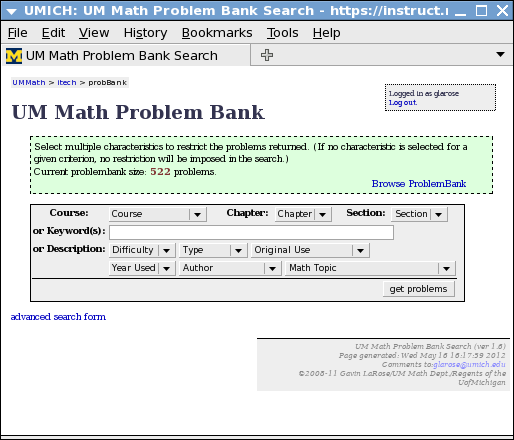
\includegraphics[height=2.5in]{um_search1}\quad
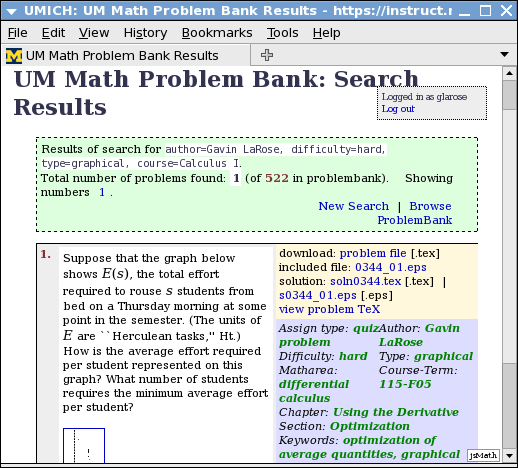
\includegraphics[height=2.5in]{um_result1}\\
\caption{UM Problem Library: left, search form; right, sample search result}
\label{umprobbank}
\end{center}
\end{figure}

The problem library in use in the mathematics department at the University
of Michigan is shown in Figure~\ref{umprobbank}, which shows the
search interface and a sample problem as displayed in a search result.
This illustrates in a general way the basic search characteristics that
will be supported by ROPE: the ability to locate problems that are
associated with specific topics in a course, which are of varying levels
of difficulty, that have specific characteristics (such as use of
graphically presented or tabular data), or which were used in specific
contexts (as homework problems, on quizzes, etc.).  This project will
dramatically rework this application, allowing it to address the goals
that are laid out in the introduction of this proposal, by including
\begin{itemize}
  \item
    scalability to support many more users, problems and problem formats,
  \item 
    community site membership and interactions,
  \item 
    problem moderation and editing,
  \item 
    problem filtering to generate alternate formats from existing
    formats,
  \item
    a modern, flexible interface that supports these features, and
  \item
    a well-documented API that will allow other applications to
    communicate with ROPE in manners other than through the browser
    interface.
\end{itemize}
These goals are described in greater detail in the following subsections.

\begin{subsection}{Scalability}

The problem library at the University of Michigan runs behind the
University web-login system and has access restricted to instructors in
the mathematics department. It accordingly supports a user base of several
hundred users, all of whom are defined by external data sources and need
no further identification or system characteristics. ROPE will support
thousands of users with internally defined characteristics (names, e-mail
addresses, password information, etc.). Accordingly, we will in the course
of the project expand the database used for the University of Michigan
system to support this. In addition, we will establish the workflow to
allow for users to author, submit and rate problems, determine the
appropriate manner in which moderation, editing of and commenting on
problems should take place, and add these functions to the problem code.

Problem types supported by the University of Michigan problem bank are
\LaTeX\ and external formats (\emph{Word} or \emph{OpenOffice} document
snippets). All problems for the problem bank are currently maintained as
separate files. For ROPE we will completely revise the problem data
structures so that all problem data are maintained in the system's
database, and completely rework the data maintained for problems to extend
the types of descriptive data for the problems and to support additional
file formats and the ability to add additional formats as they become
useful.

\end{subsection}

\begin{subsection}{Community and Site Moderation}

An aspect that is missing from the current problem bank is a mechanism for
users to provide feedback on the quality and usefulness of problems. ROPE will address this by including the ability for users to vote and
comment on problems in the library.  The data management and manner in
which this is to be done will be added to the current problembank
model.  In addition, problem view/download statistics will be provided as
part of the metadata about problems.

We will determine the nature of the voting/commenting system used, in
consultation with the Advisory Group, with the goal of maximizing its
usefulness and minimizing the possibility of any abuse. ROPE will also
support comment and problem flagging so that problems or comments with
errors can be updated by ROPE moderators. We anticipate that the moderators
will initially be drawn from the grant personnel, and will work with the
Advisory Group to determine the best manner to expand the group of people
who are engaged in this activity.  (We discuss the project's Advisory
Group in the following sections.)  ROPE will also support problem
authoring or submission from users in its community.  The degree of
moderation for this activity (if any) will also be determined by the
project personnel, including our Advisory Group.

In addition, ROPE will support a sharable problem collection feature.
This will allow users to create problem lists for their own
uses---homework sets for given courses, etc.---and to share these lists.
Thus an instructor teaching a course will be able to share her/his problem
lists with other faculty at her/his institution, or with colleagues at
other institutions.  In addition, book authors (and publishers) could
build problem lists for their texts that would then be openly available
for anyone using those texts.

\end{subsection}

\begin{subsection}{Problem Filtering}

As we add additional problem formats to ROPE, we will build in the
ability to convert between some of the formats and output types, and to
add additional filters as they are needed and developed. We anticipate
three initial filters:
\begin{itemize}
  \item
    a filter converting \TeX\ formatted problems to PDF output;
  \item
    a filter converting \TeX\ formatted problems to a rudimentary WeBWorK
    problem file; and
  \item
    a filter converting WeBWorK formatted problems to \TeX\ output. 
\end{itemize}
These will serve to provide significant additional functionality to ROPE and will be templates that illustrate the manner in which additional
filters may be constructed.

\end{subsection}

\begin{subsection}{Interface}

Considering these features and goals, it is clear that the simple search
and results interface used by the University of Michigan problem bank
system (Figure~\ref{umprobbank}) will need to be completely re-imagined.
We, with our Advisory Group, will work to develop an entirely new
interface that supports the precision of searching that we need and the
multitude of new data and features that ROPE will support.

\end{subsection}

\begin{subsection}{API and Documentation}

A natural extension to the filtering system that will be developed for ROPE is a mechanism by which other applications can use the generated
problem formats. To allow this, we will develop an easily used API by
which external applications may query ROPE to get file or problem data
for specified problems. A first application for this will be to allow the
open-source web homework system WeBWorK to include problems drawn from ROPE.  We will work with WeBWorK developers and the WeBWorK leadership
group on this aspect of the project.

\end{subsection}

\end{section}

\begin{section}{Intellectual Merit}

ROPE project will address a current need in undergraduate mathematics
education: the need for a widely available source of good problems that
instructors can use in a variety of educational venues.  Much of the
learning that takes place in mathematics, and other STEM fields, is driven
by students' work, and the success of that learning is fundamentally
dependent on the types of problems on which they work.  We therefore
expect ROPE to have the potential to be a significant and widely used
tool to enhance student learning.  

There are several specific aspects of ROPE which will have direct
bearing on this.
\begin{itemize}
  \item
    Its on-line search page that allows precise searches for specific
    types of problems.
  \item
    The open nature of the system that allows a wide range of uses of the
    problems in the library.
  \item
    The user feedback and statistics available for the problems in the
    library. 
  \item
    Users' ability to create their own problem sets, and to share
    these with other users.
  \item
    The explicitly extensible design of the system, allowing multiple
    problem formats and conversions between them.
\end{itemize}

Taking these together, we expect that ROPE will develop into an
easy-to-use, widely adopted resource with a correspondingly significant
impact on student learning of undergraduate mathematics.

\end{section}

\begin{section}{Broader Impacts}

The broad impact of ROPE will stem from its accessibility, ease-of-use
and extensibility.  We believe that the features that we are including in
ROPE will result in its use by many faculty at many institutions.  We
expect that the largest group of users of ROPE will be faculty who are
browsing for additional homework, test or quiz problems for their courses.
Even with a well-written textbook there are routine and inevitable cases
in an instructor will be at a loss to find a problem that s/he likes, and
ROPE will be the perfect resource to fill that gap.  In addition, as
open-content textbooks expand in popularity and availability, the
usefulness of ROPE will similarly increase.  We anticipate that
textbook authors may choose to define problem sets in ROPE for use by
instructors using their texts whether they are publishing open-content
textbooks or working with a publisher (though it is clear that the
attractiveness of ROPE to the former may be significantly greater).
And because ROPE will be designed from the outset to be flexible and
extensible, it will be able to meet the changing needs of faculty in the
future and make connections with other software projects for which a
library of open problems will be useful.

All told, we expect that ROPE should have very broad impact, reaching
instructors at all types of colleges and universities who are teaching any
standard mathematics course in any of a number of different ways.  We
further expect that as ROPE develops we will be able to extend it to
include other disciplines, also increasing its impact.

\end{section}
